\section{Chatbot Arena}
\label{sec:arena}

\begin{figure*}[t]
\centering
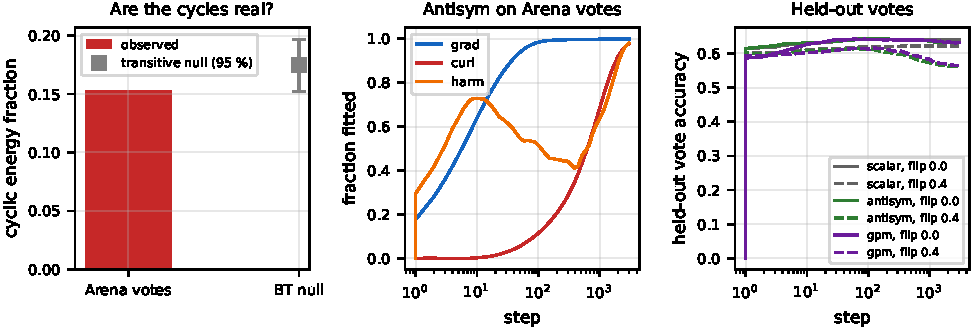
\includegraphics[width=\textwidth]{figures/arena.pdf}
\caption{Chatbot Arena, \AreItems\ models, \AreEdges\ model pairs with at
least \AreMinVotes\ votes. Left: cyclic energy of the observed log-odds flow
against a perfectly transitive Bradley--Terry null with the same counts
(median and 95\% interval). Middle: per-component fit of the antisymmetric
net under the Bradley--Terry loss. Right: held-out vote accuracy during
training, clean and with 40\% of training votes flipped (mean of seeds).}
\label{fig:arena}
\end{figure*}

We take \AreVotes\ human votes between \AreItems\ LLMs from the public Chatbot
Arena release \cite{chiang2024chatbot}, keep the \AreEdges\ model pairs with
at least \AreMinVotes\ votes, count ties as half a win, and hold out 20\% of
votes per pair (\AreHoN\ decisive held-out votes). Items have no features, so
each network sees a one-hot model identity.

\paragraph{The cycles in Arena are sampling noise.} The observed flow has
\AreFracGrad\% gradient and \AreCyc\% cyclic energy (the graph has
\AreDimCurl\ triangle dimensions and only \AreDimHarm\ harmonic ones). Is
that intransitivity? We simulate votes from the best transitive fit with the
\emph{same} per-pair counts: finite samples alone produce \AreNullCyc\% cyclic
energy (95\% interval \AreNullCycLo--\AreNullCycHi\%). The observed value sits
\emph{below} the null ($p=\AreP$ for cycles at least as strong). At the level
of models, Arena preferences show no intransitivity beyond what counting noise
creates --- which is Lemma 2 at work on real data.

\paragraph{The same order, and what it implies.} On these votes the
antisymmetric kernel ranks gradient over cycles by \AreAntisymRatio$\times$
(GPM \AreGpmRatio$\times$), and training fits the ranking by step
\AreAntisymTGrad\ and the cycles only around step \AreAntisymTCurl\
(Figure~\ref{fig:arena}, middle). Since the cycles are noise, the flexible
models' late phase is pure overfitting. Trained to the end, the scalar model is
the best held-out predictor (log-loss \AreScalarLLClean, accuracy
\AreScalarAccClean, matching HodgeRank's \AreHodgeLL\ and \AreHodgeAcc),
ahead of the antisymmetric net (\AreAntisymLLClean) and GPM (\AreGpmLLClean).
With 40\% of training votes flipped the gap widens (accuracy
\AreScalarAccFlipFour\ versus \AreAntisymAccFlipFour\ and \AreGpmAccFlipFour),
and early stopping recovers most of it (best
\AreAntisymBestFlipFour\ and \AreGpmBestFlipFour). Stopped early, a cyclic
model is a scalar model.
